\documentclass[12pt,a4paper]{article}
\usepackage[utf8]{inputenc}
\usepackage[russian]{babel}
\usepackage[left=10mm,right=10mm,top=8mm,bottom=6mm,bindingoffset=0mm]{geometry}
\usepackage{graphicx, nicefrac}
\usepackage{amsmath}
\usepackage{amsfonts}
\usepackage{amssymb}
\usepackage{multirow}
\usepackage{hhline}
\usepackage{mathtools}

\setlength{\parindent}{0em}
\setlength{\parskip}{0pt}
\setcounter{page}{0}

\graphicspath{}
\DeclareGraphicsExtensions{.pdf,.png,.jpg}
\DeclarePairedDelimiter\ceil{\lceil}{\rceil}
\DeclarePairedDelimiter\floor{\lfloor}{\rfloor}
 
\newcommand{\ds}{\displaystyle}
\newcommand{\pd}[2]{\frac{\partial #1}{\partial #2}}

\newcommand{\cc}{C_{\rm cal}}
\newcommand{\cx}{C_{\rm X}}
\newcommand{\lx}{L_{\rm X}}

\begin{document}
	\textbf{Генераторный способ измерения ёмкости и индуктивности} \\
	Заключается в измерении частоты параллельного колебательного контура (КК), состоящего из 
	индуктивности $L$ и ёмкости $C$, при параллельном подключении к нему измеряемой ёмкости $\cx$ 
	(последовательном подключении индуктивности $\lx$).
	\begin{center}
		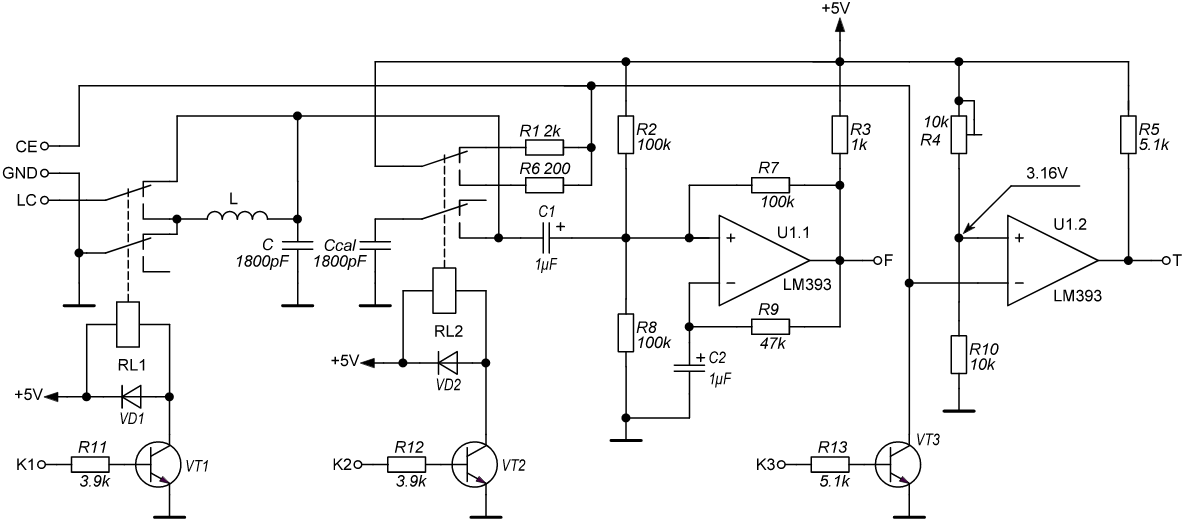
\includegraphics[scale=0.6]{sheme.png}
		Рисунок 1. схема измерительной части LC-метра.
	\end{center}	
	\textbf{Измерение ёмкости} \\
	Запишем систему уравнений для трёх, измеряемых частот:
	\begin{equation}
		\begin{cases}
			\ds \omega_1^{-2} = LC; \\[9pt]
			\ds \omega_2^{-2} = L(C+\cc); \\[9pt]
			\ds \omega_3^{-2} = L(C+\cx); \\[9pt]
		\end{cases}
	\end{equation}
	где $\ds\omega_n=2\pi f_n$ - измеряемые частоты КК.
	$\ds f_1$ -- частота исходного КК,
	$\ds f_2$ -- частота КК с параллельно подключенным 
	калибровочным конденсатором -- $\ds\cc$,
	$\ds f_3$ -- частота КК с параллельно подключенным 
	измеряемым конденсатором -- $\ds\cx$.
	После следующих преобразований системы (1): \\
	\begin{equation*}
	\begin{cases}
		\ds \omega_2^{-2} = LC + L\cc = \omega_1^{-2} + L\cc; \\[9pt]
		\ds \omega_3^{-2} = LC + L\cx = \omega_1^{-2} + L\cx; \\[9pt]
	\end{cases} \quad
	\begin{cases}
		\ds L = \frac{\omega_2^{-2} - \omega_1^{-2}}{\cc}; \\[9pt]
		\ds \omega_3^{-2} = \omega_1^{-2} + L\cx = 
		\omega_1^{-2} + \frac{\cx}{\cc}(\omega_2^{-2} - \omega_1^{-2}); \\[9pt]
	\end{cases}
	\end{equation*}
	$\ds \frac{\cx}{\cc}(\omega_2^{-2} - \omega_1^{-2}) = \omega_3^{-2} - \omega_1^{-2}; \quad
	\frac{\cx}{\cc} = \frac{\omega_3^{-2} - \omega_1^{-2}}{\omega_2^{-2} - \omega_1^{-2}} =
	\frac{\ds\frac{\omega_3^{-2}}{\omega_1^{-2}} - 1}{\ds\frac{\omega_2^{-2}}{\omega_1^{-2}} - 1} =
	\frac{{\left(\ds\frac{\omega_1}{\omega_3}\right)}^2 - 1}{{\left(\ds\frac{\omega_1}{\omega_2}\right)}^2 - 1}; \quad
	\cx = \frac{{\left(\ds\frac{2\pi f_1}{2\pi f_3}\right)}^2 - 1}{{\left(\ds\frac{2\pi f_1}{2\pi f_2}\right)}^2 - 1} \cdot \cc;$ \\[5pt]
	получаем формулу для вычисления $\cx$ через измеренные частоты: $f_1, f_2, f_3$ и значение ёмкости
	калибровочного конденсатора $\cc$, которые считаются известным:
	\begin{equation}
		\ds \cx = \frac{{\left(\ds\frac{f_1}{f_3}\right)}^2 - 1}{{\left(\ds\frac{f_1}{f_2}\right)}^2 - 1} \cdot \cc;
	\end{equation}
	\newpage
	\textbf{Измерение индуктивности} \\
	Получим формулу для вычисления измеряемой индуктивности $\lx$. 
	Запишем систему уравнений для трёх, измеряемых частот: \\
	\begin{equation}
		\begin{cases}
			\ds \omega_1^{-2} = LC; \\[9pt]
			\ds \omega_2^{-2} = L(C+\cc); \\[9pt]
			\ds \omega_3^{-2} = (L+\lx)C; \\[9pt]
		\end{cases}
	\end{equation}
	где $\ds f_3$ -- частота КК с последовательно подключенной 
	измеряемой индуктивностью -- $\ds\lx$.
	После следующих преобразований системы (3): \\
	\begin{equation*}
		\begin{cases}
			\ds L = \frac{\omega_1^{-2}}{C}; \\[9pt]
			\ds \omega_2^{-2} = \frac{\omega_1^{-2}}{C}(C+\cc); \\[9pt]
			\ds \omega_3^{-2} = \left(\frac{\omega_1^{-2}}{C}+\lx\right)C; \\[9pt]
		\end{cases} \Rightarrow \quad
		\begin{cases}
			\ds \omega_2^{-2} - \omega_1^{-2} = \frac{\omega_1^{-2}}{C}\cdot\cc; \\[9pt]
			\ds \omega_3^{-2} - \omega_1^{-2} = \lx C; \\[9pt]
		\end{cases} \Rightarrow \quad
		\begin{cases}
			\ds \frac{\omega_2^{-2}}{\omega_1^{-2}} - 1 = \frac{\cc}{C}; \\[9pt]
			\ds \frac{\omega_3^{-2}}{\omega_1^{-2}} - 1 = \lx\frac{C}{\omega_1^{-2}}; \\[9pt]
		\end{cases}
	\end{equation*}
	\begin{equation*} 
		\begin{cases}
			\ds \frac{\cc}{C} = \frac{\omega_2^{-2}}{\omega_1^{-2}} - 1; \\[9pt]
			\ds \lx = \left(\frac{\omega_3^{-2}}{\omega_1^{-2}} - 1\right)\frac{\omega_1^{-2}}{C}; \\[9pt]
		\end{cases} \Rightarrow \quad
		\begin{cases}
			\ds \frac{1}{C} = \left[{\left(\frac{\omega_1}{\omega_2}\right)}^2 - 1\right]\frac{1}{\cc}; \\[12pt]
			\ds \lx = \left[{\left(\frac{\omega_1}{\omega_3}\right)}^2 - 1\right]\frac{1}{\omega_1^2C}; \\[12pt]
		\end{cases}
	\end{equation*}
	\begin{equation*}
		\ds \lx = \left[{\left(\frac{\omega_1}{\omega_3}\right)}^2 - 1\right]\left[{\left(\frac{\omega_1}{\omega_2}\right)}^2 - 1\right]\frac{1}{\omega_1^2\cc};
	\end{equation*}
	имеем формулу для вычисления индуктивности $\lx$:
	\begin{equation}
		\ds \lx = \left[{\left(\frac{f_1}{f_3}\right)}^2 - 1\right]\left[{\left(\frac{f_1}{f_2}\right)}^2 - 1\right]\frac{1}{4\pi^2f_1^2\cc};
	\end{equation}
	\\
	\textbf{Калибровка} \\
	Калибровка измерительного контура заключается в 
	предварительном измерении частот $f_1$ и $f_2$.
	Откуда с помощью следующих преобразований двух
	первых уравнений системы (1): \\
	\begin{equation*}
		\begin{cases}
			\ds \omega_1^{-2} = LC; \\[9pt]
			\ds \omega_2^{-2} = L(C+\cc); \\[9pt]
		\end{cases} \Rightarrow \quad
		\begin{cases}
			\ds L = \frac{\omega_1^{-2}}{C}; \\[9pt]
			\ds \frac{\omega_2^{-2}}{L} = C+\cc; \\[9pt]
		\end{cases} \Rightarrow \quad
		\begin{cases}
			\ds L = \frac{\omega_1^{-2}}{C}; \\[9pt]
			\ds C\frac{\omega_2^{-2}}{\omega_1^{-2}} = C+\cc; \\[9pt]
		\end{cases}
		\ds C\left(\frac{\omega_1^2}{\omega_2^2}-1\right) = \cc;
	\end{equation*}
	получим формулу для вычисления ёмкости $C$: \\
	\begin{equation}
		\ds C = \frac{\cc}{{\left(\ds\frac{\omega_1}{\omega_2}\right)}^2-1} =
		\frac{1}{{\left(\ds\frac{f_1}{f_2}\right)}^2-1}\cdot\cc;
	\end{equation}
	а также после следующих преобразований: \\
	\begin{equation*}
		\begin{cases}
			\ds \omega_1^{-2} = LC; \\[9pt]
			\ds \omega_2^{-2} = L(C+\cc); \\[9pt]
		\end{cases} \Rightarrow \quad
		\begin{cases}
			\ds C = \frac{\omega_1^{-2}}{L}; \\[9pt]
			\ds L = \frac{\omega_2^{-2}}{C+\cc}; \\[9pt]
		\end{cases}
		\ds L = \frac{\omega_2^{-2}}{\ds\frac{\omega_1^{-2}}{L}+\cc}; \quad
		\frac{\omega_1^{-2}}{L}+\cc = \frac{\omega_2^{-2}}{L};
	\end{equation*}
	\begin{equation*}
		\ds \frac{\omega_2^{-2}-\omega_1^{-2}}{L} = \cc; \quad
		L = \frac{\omega_2^{-2}-\omega_1^{-2}}{\cc} = 
		\frac{1}{\cc}\left(\frac{1}{\omega_2^2}-\frac{1}{\omega_1^2}\right) =
		\frac{1}{\cc}\cdot\frac{\omega_1^2-\omega_2^2}{\omega_1^2\omega_2^2} =
		\frac{\ds\frac{\omega_1^2}{\omega_2^2}-1}{\omega_1^2}\cdot\frac{1}{\cc};
	\end{equation*}
	получаем формулу для вычисления индуктивности $L$: \\
	\begin{equation}
		\ds L = \left[{\left(\frac{\omega_1}{\omega_2}\right)}^2-1\right]\frac{1}{\omega_1^2\cc} =
		\left[{\left(\frac{f_1}{f_2}\right)}^2-1\right]\frac{1}{4\pi^2f_1^2\cc};
	\end{equation}
	\\
	Сравнивая (2) с (5) и (4) с (6) легко видеть, 
	что обе пары формул отличаются множителем: \\
	\begin{equation*}
		\ds {\left(\frac{f_1}{f_3}\right)}^2 - 1
	\end{equation*}
	то есть после калибровки для $\cx$ и $\lx$ справедливы следующие формулы:
	\begin{equation} 
		\begin{cases}
			\ds \cx = \left[{\left(\frac{f_1}{f_3}\right)}^2 - 1\right]C; \\[12pt]
			\ds \lx = \left[{\left(\frac{f_1}{f_3}\right)}^2 - 1\right]L; \\[12pt]
		\end{cases}
	\end{equation}
	\\
	\textbf{Измерение ёмкости электролитических конденсаторов 
	через постоянную времени} \\
	Измеряемый конденсатор $C_E$ заряжается через известное 
	сопротивление $R$ по закону: \\
	\begin{equation} 
		\ds U_C(t) = U_0\left[1-\exp\left(-\frac{t}{RC_E}\right)\right];
	\end{equation}
	где $U_C(t)$ -- напряжение на конденсаторе $C_E$, 
	$U_0$ -- напряжение источника питания.
	Измеряя время $t$, за которое измеряемый конденсатор 
	зарядится от $0$ до напряжения $U_0/2$,
	можно вычислить ёмкость $C_E$: \\
	\begin{equation*} 
		\ds \frac12U_0 = U_0\left[1-\exp\left(-\frac{t}{RC_E}\right)\right];
	\end{equation*}
	\begin{equation*} 
		\ds \frac12 = 1-\exp\left(-\frac{t}{RC_E}\right);
	\end{equation*}
	\begin{equation*} 
		\ds -\frac12 = -\exp\left(-\frac{t}{RC_E}\right);
	\end{equation*}
	\begin{equation*} 
		\ds \ln\left(\frac12\right) = -\frac{t}{RC_E};
	\end{equation*}
	\begin{equation*} 
		\ds -\ln(2) = -\frac{t}{RC_E};
	\end{equation*}
	\begin{equation*} 
		\ds \ln(2) = \frac{t}{RC_E};
	\end{equation*}
	\begin{equation} 
		\ds C_E = \frac{t}{R\ln(2)} \approx \frac{t}{0.693R};
	\end{equation}
	Если настроить комапаратор на напряжение:
	\begin{equation*} 
		\ds U_{\rm REF} = \left(1-\frac1e\right)U_0,
	\end{equation*}
	то формула (9) упроститься до:
	\begin{equation} 
		\ds C_E = \frac{t}{R};
	\end{equation}
	\newpage
	\textbf{Измерение временных интервалов, а равно и частоты 
	с помощью микроконтроллера} \\
	Пусть имеется два таймера: TMR1 --- таймер-счётчик и 
	TMR2 --- таймер.
	Таймер TMR1 -- тактируется измеряемой частотой $f$ и 
	хранит в своём счётном регистре $T_1$ количество импульсов, 
	поступивших на его тактовый вход. 
	Таймер TMR2 -- отсчитывает интервалы времени и содержит в
	своём счётном регистре $T_2$ число пропорциональное 
	времени между его включением и остановкой. 
	Интервал времени вычислется по формуле: \\
	\begin{equation} 
		\ds \Delta T = \frac{k}{f_{\rm CLK}}\cdot T_2,
	\end{equation}
	где $k$ --- коэффициент предделителя таймера, $f_{\rm CLK}$ ---
	частота тактирования таймера.
	Таймер TMR2 отсчитывает интервалы времени $\Delta T$ в течении которых
	таймер TMR1 считает импульсы измеряемого сигнала. Частота вычисляется
	как:
	\begin{equation} 
		\ds f = \frac{T_1}{\Delta T} = 
		\frac{T_1}{T_2}\cdot\frac{f_{\rm CLK}}{k}.
	\end{equation}
\end{document}
